% Classic HLS DSE overview (content = two reference figures; layout cleaned)
\documentclass[tikz,border=4pt]{standalone}
\usepackage{times}
\usepackage{xcolor}
\usetikzlibrary{arrows.meta,calc}

\definecolor{cOpt}{RGB}{225,205,240}
\definecolor{cTech}{RGB}{255,218,185}
\definecolor{cSrc}{RGB}{255,205,165}
\definecolor{cHLS}{RGB}{175,220,185}
\definecolor{cImpl}{RGB}{175,210,245}
\definecolor{cLay}{RGB}{245,228,175}
\definecolor{cExp}{RGB}{238,238,238}
\definecolor{cPareto}{RGB}{248,252,255}
\definecolor{cSub}{RGB}{255,255,255}
\definecolor{cBorder}{RGB}{45,45,45}
\definecolor{cAxis}{RGB}{195,55,45}
\definecolor{cFront}{RGB}{35,85,175}

\begin{document}
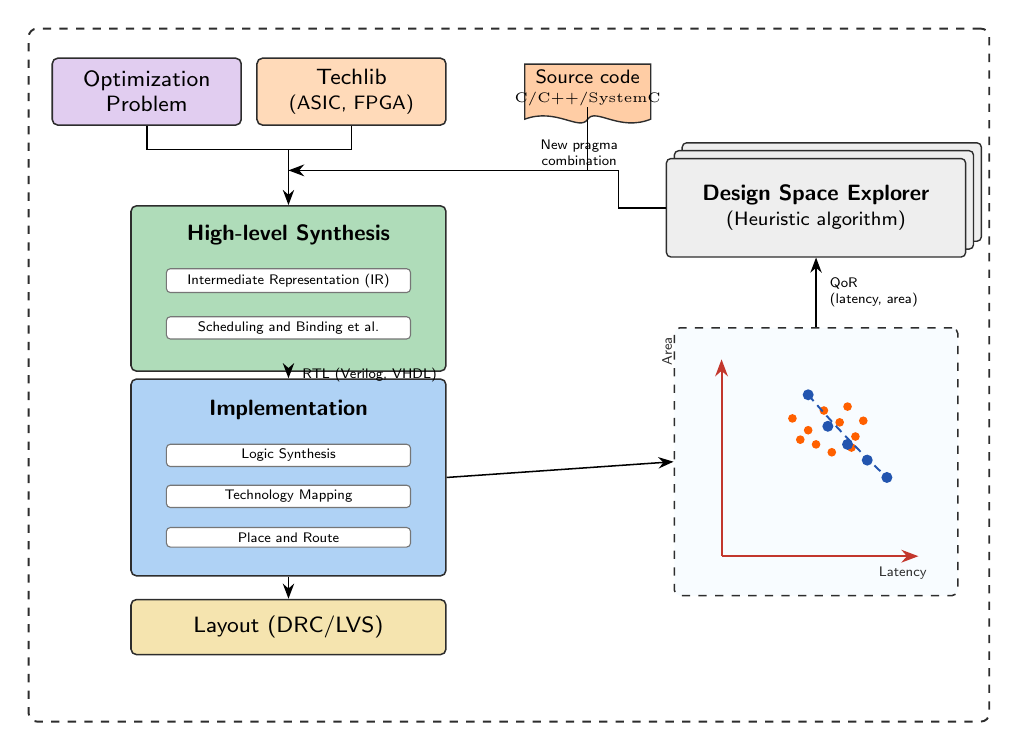
\begin{tikzpicture}[
  >=Stealth,
  font=\sffamily\footnotesize,
  box/.style={
    draw=cBorder, rounded corners=2pt, align=center,
    inner sep=2.8pt, line width=0.55pt
  },
  sub/.style={
    draw=cBorder!65, fill=cSub, rounded corners=1.4pt,
    font=\sffamily\tiny, inner sep=1.8pt, align=center,
    minimum width=31mm, line width=0.4pt
  },
]

% ---- canvas / frame ----
\node[draw=cBorder, dashed, line width=0.7pt, rounded corners=3pt,
  minimum width=122mm, minimum height=88mm] (frame) at (0,-1mm) {};

% ================= TOP INPUTS =================
\node[box, fill=cOpt, minimum width=24mm, minimum height=8.5mm] (opt)
  at (-46mm, 35mm) {Optimization\\[-0.4pt]Problem};

\node[box, fill=cTech, minimum width=24mm, minimum height=8.5mm] (tech)
  at (-20mm, 35mm) {Techlib\\[-0.4pt]{\scriptsize(ASIC, FPGA)}};

\begin{scope}[shift={(2mm,35.5mm)}]
  \filldraw[fill=cSrc, draw=cBorder, line width=0.5pt]
    (0,3mm) -- (16mm,3mm) -- (16mm,-4mm)
    .. controls (12mm,-5.6mm) and (9mm,-2.5mm) .. (8mm,-4mm)
    .. controls (7mm,-5.6mm) and (4mm,-2.5mm) .. (0,-4mm) -- cycle;
  \node[align=center, font=\sffamily\scriptsize] at (8mm,0)
    {Source code\\[-1pt]{\normalfont\tiny C/C++/SystemC}};
\end{scope}
\coordinate (src) at (10mm, 33mm);

% feed rail above HLS
\coordinate (rail) at (-28mm, 25mm);

% ================= LEFT PIPELINE =================
\node[box, fill=cHLS, minimum width=40mm, minimum height=21mm] (hls)
  at (-28mm, 10mm) {};
\node[font=\sffamily\footnotesize\bfseries]
  at ([yshift=6.8mm]hls.center) {High-level Synthesis};
\node[sub] at ([yshift=1.0mm]hls.center) {Intermediate Representation (IR)};
\node[sub] at ([yshift=-5.0mm]hls.center) {Scheduling and Binding et al.};

\node[box, fill=cImpl, minimum width=40mm, minimum height=25mm] (impl)
  at (-28mm, -14mm) {};
\node[font=\sffamily\footnotesize\bfseries]
  at ([yshift=8.6mm]impl.center) {Implementation};
\node[sub] at ([yshift=2.8mm]impl.center) {Logic Synthesis};
\node[sub] at ([yshift=-2.4mm]impl.center) {Technology Mapping};
\node[sub] at ([yshift=-7.6mm]impl.center) {Place and Route};

\node[box, fill=cLay, minimum width=40mm, minimum height=7mm] (lay)
  at (-28mm, -33mm) {Layout (DRC/LVS)};

% ================= RIGHT: Explorer =================
\begin{scope}
  \foreach \o in {2.0, 1.0, 0} {
    \filldraw[fill=cExp, draw=cBorder, line width=0.5pt, rounded corners=1.6pt]
      ({20mm+\o mm},{14mm+\o mm}) rectangle ++(38mm,12.5mm);
  }
\end{scope}
\node[align=center, minimum width=38mm, minimum height=12.5mm] (exp)
  at (39mm, 20.25mm)
  {\textbf{Design Space Explorer}\\[-0.3pt]
   {\scriptsize(Heuristic algorithm)}};

% ================= Pareto =================
\begin{scope}[shift={(39mm,-12mm)}]
  \node[draw=cBorder, dashed, line width=0.55pt, rounded corners=2pt,
    fill=cPareto, minimum width=36mm, minimum height=34mm] (pareto) {};
  \draw[->, cAxis, line width=0.7pt] (-12mm,-12mm) -- (13mm,-12mm)
    node[below, font=\sffamily\tiny, text=cBorder, xshift=-2mm]{Latency};
  \draw[->, cAxis, line width=0.7pt] (-12mm,-12mm) -- (-12mm,13mm)
    node[above, font=\sffamily\tiny, text=cBorder, rotate=90,
      yshift=5mm, xshift=1mm]{Area};
  \foreach \x/\y in {-3/5.5, -1/4, 1/6.5, 0/2.2, 3/5, 4/7, 2/1.2, 5/3.2, 6/5.2, -2/2.8, 4.5/1.8} {
    \fill[orange!75!red] (\x mm, \y mm) circle (0.55mm);
  }
  \foreach \x/\y in {-1/8.5, 1.5/4.5, 4/2.2, 6.5/0.2, 9/-2} {
    \fill[cFront] (\x mm, \y mm) circle (0.7mm);
  }
  \draw[cFront, densely dashed, line width=0.7pt]
    (-1mm,8.5mm) .. controls (2mm,5mm) and (5mm,1.8mm) .. (9mm,-2mm);
\end{scope}

% ================= ARROWS =================
% three inputs → rail → HLS  (keep clear of Explorer)
\draw[-, line width=0.55pt] (opt.south) -- ++(0,-3mm) -| (rail);
\draw[-, line width=0.55pt] (tech.south) -- ++(0,-3mm) -| (rail);
\draw[-, line width=0.55pt] (src) |- (rail);
\draw[->, line width=0.55pt] (rail) -- (hls.north);

% HLS → Impl → Layout
\draw[->, line width=0.55pt]
  (hls.south) --
  node[right, font=\sffamily\tiny, xshift=0.5mm]{RTL (Verilog, VHDL)}
  (impl.north);
\draw[->, line width=0.55pt] (impl.south) -- (lay.north);

% Impl → Pareto
\draw[->, line width=0.55pt] (impl.east) -- (pareto.west);

% Pareto → Explorer (QoR)
\draw[->, line width=0.55pt]
  (pareto.north) --
  node[right, font=\sffamily\tiny, align=left, xshift=0.5mm]
  {QoR\\(latency, area)}
  (exp.south);

% Explorer → New pragma → rail (gap between pipeline and explorer)
\draw[->, line width=0.6pt]
  (exp.west) -- ++(-6mm,0) |- (rail);
\node[font=\sffamily\tiny, align=center]
  at ($(exp.west)+(-11mm,7mm)$) {New pragma\\combination};

\end{tikzpicture}
\end{document}
